\documentclass[11pt]{article}

\usepackage{amsfonts}
\usepackage{amssymb}
\usepackage{amsthm}
\usepackage{fancybox}
\usepackage{amsmath}
\usepackage{fullpage}
\usepackage{setspace}
\usepackage{mathtools}
\usepackage{times}
\usepackage{color}
\usepackage{hyperref}
\usepackage{polynom}
\usepackage[utf8]{inputenc}

\usepackage[pdftex]{graphicx}
\usepackage{multicol}
\usepackage{fancyhdr}
\usepackage{titlesec}

\setlength{\fboxsep}{1em}
\setlength{\parindent}{0pt}
\setlength{\headheight}{14pt}
\renewcommand{\headrulewidth}{1pt}
\renewcommand{\footrulewidth}{1pt}
\setlength{\headsep}{14pt}

\begin{document}

\pagestyle{fancy}
\fancyhead{}
\fancyhead[L]{CSCC43}
\fancyhead[R]{PROJECT:\@MyBnB}
\fancyfoot{}
\fancyfoot[R]{\thepage}
\fancyfoot[L]{Pasa Ali Aslan}

\section*{Project Description}

MyBnB is a home sharing service platform like AirBnb in which users can list or book
residences around the world. Recognizing its mass audience, MyBnB is planned to be
a full-stack application with web and mobile support.

Considering course objectives and limited time-frame, this project (its source code)
aims to provide the HTTP server (Java) and database (MySQL) portion of MyBnB with minimal functionality given by the
project requirements. Similarly, Java SQL adapters are used with raw MySQL queries
to enable the developer to strenthen his understanding on the database transactions. No frameworks or ORMs are used and
most if not all resulting tables from the SQL queries are returned directly as HTTP response (i.e.
most operations including but not limited to sorting, filtering, etc., are done through SQL).
Nevertheless, the server code is written as systematically as possible to keep a consistent high code
quality.


\section*{Source Code and Setup}

The source code can be found in https://github.com/pasaaliaslan/mybnb. `README.md' provides all the necessary
information (or references the documents with the specific information), including the setup
process on a local machine, server API documentation, and blueprints of the database system
(ER diagrams, schemas, assumptions, etc.).

After one completes the setup process, he can run HTTP queries on terminal or (more simply)
on Postman. Each endpoint is well documented under `./doc/apis'

\section*{Assumptions}

\begin{itemize}
\item Country, Subcountry, and City tables are prepopulated as they are static (unless new countries, subcountries, and cities are established).
User will choose one of the country, subcountry, city from the rows defined in these tables (i.e., no chance for user to input country/subcountry/city, eliminating the possibility of having inaccurate data).

\item Ideally, postal code should have been static too. However, due to the small extent of this project, millions of postal codes are not put into a table and it is assumed that the users will enter valid postal codes for their addresses.

\item It is assummed that street name and coordinate data matches with country/subcountry/city data inputted by the user.

\end{itemize}

\newpage
\section*{ER Diagram}

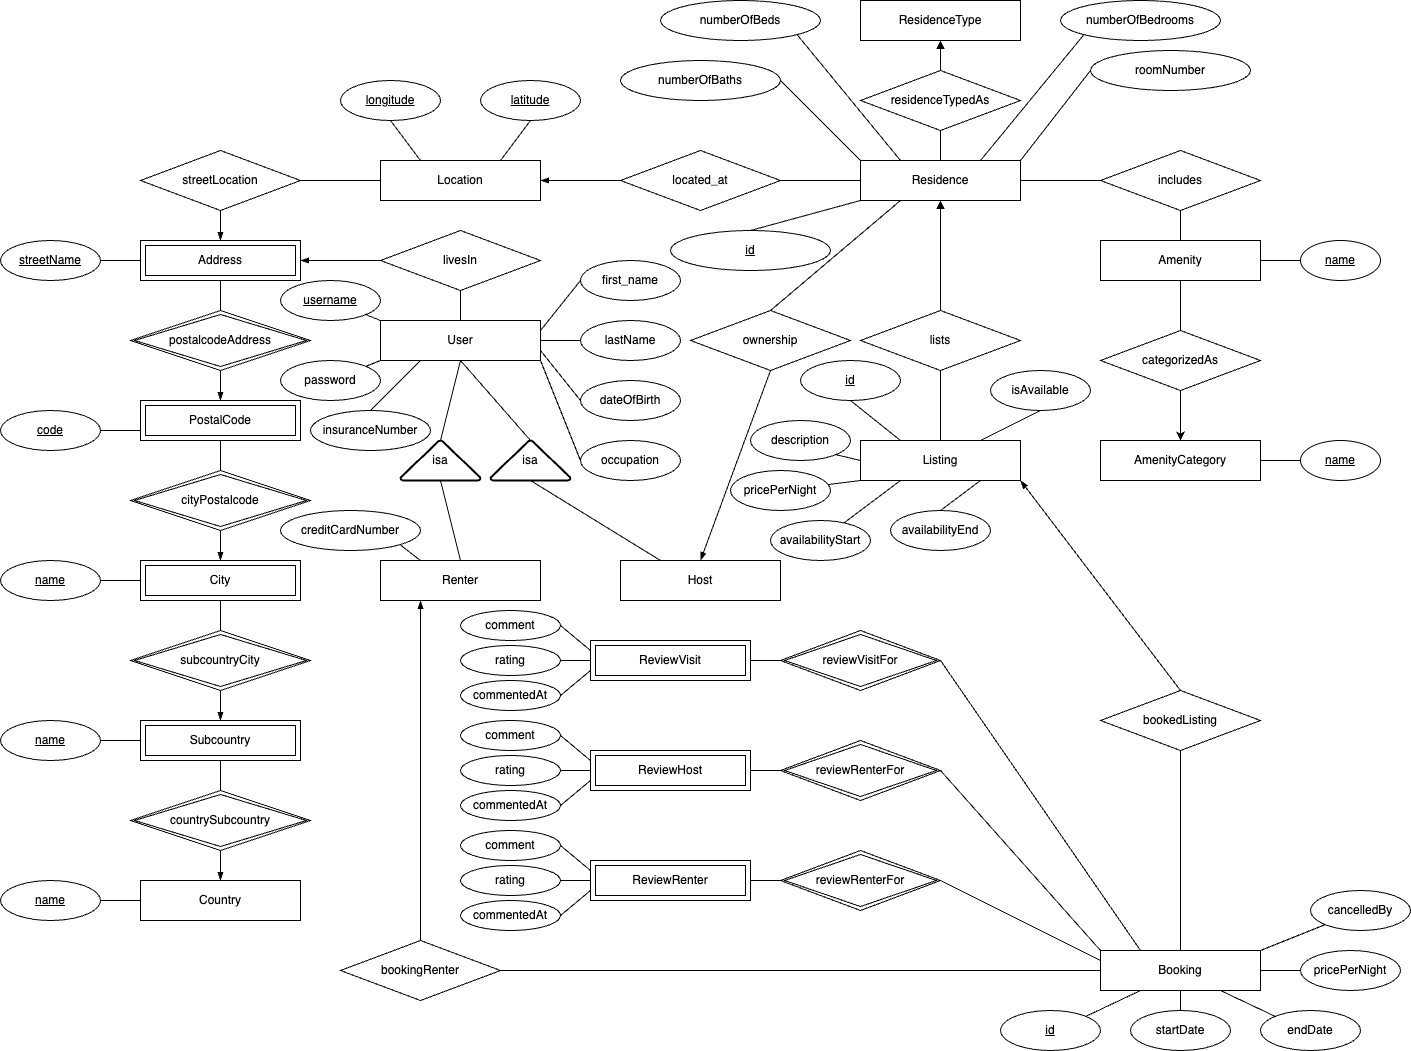
\includegraphics[scale=0.35]{er}

\newpage
\section*{Schemas}

Country (\underline{name})

Subcountry (\underline{name}, \underline{countryName})

City (\underline{name}, \underline{subcountryName}, \underline{countryName})

PostalCode (\underline{code}, \underline{cityName}, \underline{subcountryName}, \underline{countryName})

Address (\underline{streetName}, \underline{postalCode}, \underline{cityName}, \underline{subcountryName}, \underline{countryName})

Location (\underline{longitude}, \underline{latitude}, streetName, postalCode, cityName, subcountryName, countryName)

User (\underline{username}, password, insuranceNumber, firstName, lastName, dateOfBirth, occupation)

livesIn (\underline{username}, streetName, postalCode, cityName, subcountryName, countryName)

Renter (\underline{username}, creditCardNumber)

Host (\underline{username})

ResidenceType(\underline{name})

Residence(\underline{id}, residenceTypeName,hostUsername,numberOfBedrooms, numberOfBeds, numberOfBaths, roomNumber, longitude, latitude)

Listing (\underline{id}, description, pricePerNight, availabilityStart, availabilityEnd, residenceId, isAvailable)

AmenityCategory (\underline{name})

Amenity (\underline{name}, amenityCategoryName)

includes (\underline{residenceId}, \underline{amenityName})

Booking (\underline{id}, startDate, endDate, renterUsername, listingId, pricePerNight, cancelledBy)

reviewHost (\underline{commentedAt}, \underline{bookingId}, comment, rating)

reviewRenter (\underline{commentedAt},  \underline{bookingId}, comment, rating)

reviewVisit (\underline{commentedAt}, \underline{bookingId}, comment, rating)

\section*{Constraints}
\begin{itemize}
  \item User
  \begin{itemize}
    \item The difference between dateOfBirth and TODAY should be at least 18 years.
  \end{itemize}
  \item Listing
  \begin{itemize}
    \item availabilityStart $\leq$ availabilityEnd.
    \item A residence can have multiple listings, but none of the listings for the same residence have overlapping availability range.
  \end{itemize}
  \item Booking
  \begin{itemize}
    \item startDate $\leq$ endDate.
    \item Start and end date of a booking is within the availability range of the listing that is booked.
    \item No two bookings refer to same listing if their date range overlap.
  \end{itemize}
  \item ReviewHost, ReviewVisit, ReviewRenter.
  \begin{itemize}
    \item Rating should be between 1 and 5 (inclusive).
    \item A review can be made after the visit is completed.
    \item A review cannot be made in future.
  \end{itemize}
\end{itemize}


\newpage

\section*{Limitations and Areas of Improvement}

\begin{enumerate}
  \item Country, Subcountry, and City tables are prepopulated to prevent multiple rows
  for the same entry (e.g., `toronto' and `Toronto' most likely refer to same city).
  Prepopulation is possible because the dataset is already provided and a subject to
  little or change in the long run (i.e., country/subcountry/city names change infrequently
  if not never.). Similarly, PostalCode field could have been prepopulated to further
  improve consistency, especially when the algorithm for price suggestion is considered.

  \item There is a chance for a coordinate value to not match with the address. There is no
  way to prevent this issue on the database layer, but external APIs can be utilized to ensure
  coordinate values match the address.

  \item Error handling on the server level is minimal, putting responsibility to the
  potential frontend level of the application. Server provides some helper viewsets
  to assist frontend in this regard. For instance, Country viewset yields the full list
  of countries stored in the Country table of the database, so that the frontend could
  serve this list as options (like a dropdown component) and prevent users from inputting
  invalid values.

  \item There is no authentication implemented in the server. Hence, anyone can call any
  endpoint, which is not ideal when the host/user hierarchy is considered. Simple token/session
  can be implemented to solve endpoint access issues entirely.

  \item Key properties cannot be updated in MyBnB. For instance, as `username' is key
  of `User' table, one cannot simply change his/her username. There are various reasons for this
  design choice. First of all, as all updates are applied on non-key properties, it is guaranteed
  to not update any foreign references (assuming design follows normal forms). Thus, the update
  occurs only in the original table and nowhere else. Also, foreign references can break among
  different tables and rows if key properties could be updated. For instance, assume we have users
  A and B who lives in the same address. Hence, User A and User B both refer to same row in the
  `Address' table through `livesIn' table. Let User A change his address (i.e. key in `Address' table).
  As A and B were refering the same row, the system would change the address of B too, which
  is not the case.

  \item Price/amenity suggestion algorithm can be improved significantly by including different parameters
  such as availability date range of the listing, number of baths/beds/bedrooms in the residence,
  multivariable impacts of each amenity, etc.
\end{enumerate}


\end{document}
